\documentclass[tikz]{standalone}
%\usetikzlibrary{calc}
\begin{document}


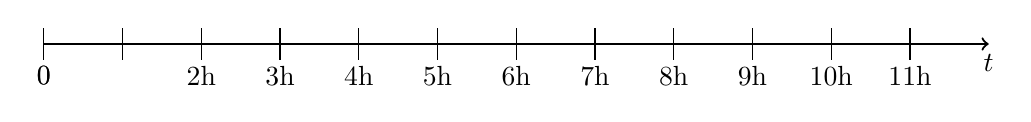
\begin{tikzpicture}[node distance=3cm]
  \draw[->, thick] (0,0)  -- node [below, at end] {$t$} (12,0);

  \def\samples{11}
  \def\samplperiod{1} 
  \def\ticksize{0.2}

  \draw (0, -\ticksize) -- (0, \ticksize);
  \node at (0, -2*\ticksize) {$0$};
  \draw (\samplperiod, -\ticksize) -- (\samplperiod, \ticksize);
  \node at (0, -2*\ticksize) {$0$};

\foreach \k in {2,...,\samples}
{
  \draw (\k*\samplperiod, -\ticksize) -- (\k*\samplperiod, \ticksize);

  \node at (\k*\samplperiod, -2*\ticksize) {\k h};
}
\end{tikzpicture}
\end{document}
